% !TEX program = xelatex

\documentclass[12pt,a4paper]{article}
\usepackage[UTF8]{ctex}
\usepackage{float}
\usepackage{amsmath}
\usepackage{amsfonts}
\usepackage{enumerate}
\usepackage{booktabs}
\usepackage{graphicx}
\usepackage{longtable}
\usepackage{subfigure}

\usepackage{url}
\usepackage{multirow}

% for plotting 
\usepackage{caption}
\usepackage{pgfplots}

% for pseudo code 
\usepackage{algorithm}
\usepackage[noend]{algpseudocode}

% for reference 
\usepackage{hyperref}
\usepackage{cleveref}

% for code 
\usepackage{listings}
\usepackage{xcolor}
\usepackage{fontspec}
\definecolor{darkgreen}{rgb}{0,0.6,0}
\newfontfamily\consolas{Consolas}

\usepackage{amssymb}
\usepackage{pifont}
\usepackage{xcolor}
\newcommand{\cmark}{\ding{51}}
\newcommand{\xmark}{\ding{55}}

\lstset {
    basicstyle=\footnotesize\consolas, % basic font setting
    breaklines=true, 
    frame=single,     % {single, shadowbox, bottomline}
    keywordstyle=\color{blue}, 
    commentstyle=\color{darkgreen},
    stringstyle=\color{red},
    showstringspaces=false,
    % backgroundcolor=\color{black!5}, % set backgroundcolor
    numbers=left, 
    numberstyle=\ttfamily,
}

% Microsoft Word A4 paper default layout 
\usepackage[a4paper, left=3.18cm, right=3.18cm, top=2.54cm, bottom=2.54cm]{geometry}

% \captionsetup[figure]{labelfont={bf}, name={Figure}}
% \captionsetup[table]{labelfont={bf}, name={Table}}

\crefname{equation}{方程}{方程}
\Crefname{equation}{方程}{方程}
\crefname{table}{表}{表}
\Crefname{table}{表}{表}
\crefname{figure}{图}{图}
\Crefname{figure}{图}{图}

\title{数学实验:第十次作业}
\author{计算机系 \quad 计73 \quad 2017011620 \quad 李家昊}
\date{\today}

% 实验报告格式的基本要求

% 系别、班级、学号、姓名

% 1 实验目的
% 2 题目
%   2.1 计算题:题号,算法设计(包括计算公式),程序,计算结果(计算机输出),结果分析,结论。
%   2.2 应用题:题号,问题分析,模型假设,模型建立,算法设计(包括计算公式),程序,计算结果(计算机输出),结果的数学分析,结果的实际意义,结论。
% 3 收获与建议

% Calc
% \subsubsection{算法设计}
% \subsubsection{程序}
% \subsubsection{计算结果}
% \subsubsection{结果分析}
% \subsubsection{结论}

% App
% \subsubsection{问题分析}
% \subsubsection{模型假设}
% \subsubsection{模型建立}
% \subsubsection{算法设计}
% \subsubsection{程序}
% \subsubsection{计算结果}
% \subsubsection{结果的数学分析}
% \subsubsection{结果的实际意义}
% \subsubsection{结论}

\begin{document}

\maketitle

\section{实验目的}

\begin{itemize}
    \item 了解回归分析的基本原理,掌握MATLAB实现的方法。
    \item 练习用回归分析解决实际问题。
\end{itemize}

\section{问题求解}

\subsection{Chap13-Ex7 有氧锻炼(计算题)}

\subsubsection{算法设计}

\paragraph{模型建立} 记报童每天购入报纸数量为$n$,需求量为$r$,服从正态分布$N(\mu, \sigma^2)$,其概率密度函数为$f$,批发价为$a=A(1-n/K)$,每份报纸的零售价为$b$,退回价为$c$,则报童每天的利润$V$为,
\begin{equation}\label{eq:ex7_profit}
    V(n)=\sum_{r=0}^{n-1}[(b-a) r-(a-c)(n-r)] f(r)+\sum_{r=n}^{\infty}[(b-a) n] f(r)
\end{equation}

其图像如\Cref{fig:ex7_profit},可以看到,随着购入报纸数量$n$的增大,利润$V$首先在$n=2000$附近出现了一个极大值,然后降低到负值,然而,随着$n$的继续增大,$V$的值出现了急速的攀升,甚至超过了之前的极大值。这是因为随着$n$的增大,批发价格$a$逐渐降低,当$n>15000$时,批发价格竟然低于回收价格,当$n>50000$时,批发价格甚至变成了负数,在这些情况下,报童只要多购进报纸,再统一进行回收,就能赚到差价,显然是不符合实际情况的。为了保证批发价与回收价之间有一定的差价,这里对$n$的范围做如下规定,
\begin{equation}
    0 \le n \le 5000
\end{equation}

\begin{figure}[H]
    \centering
    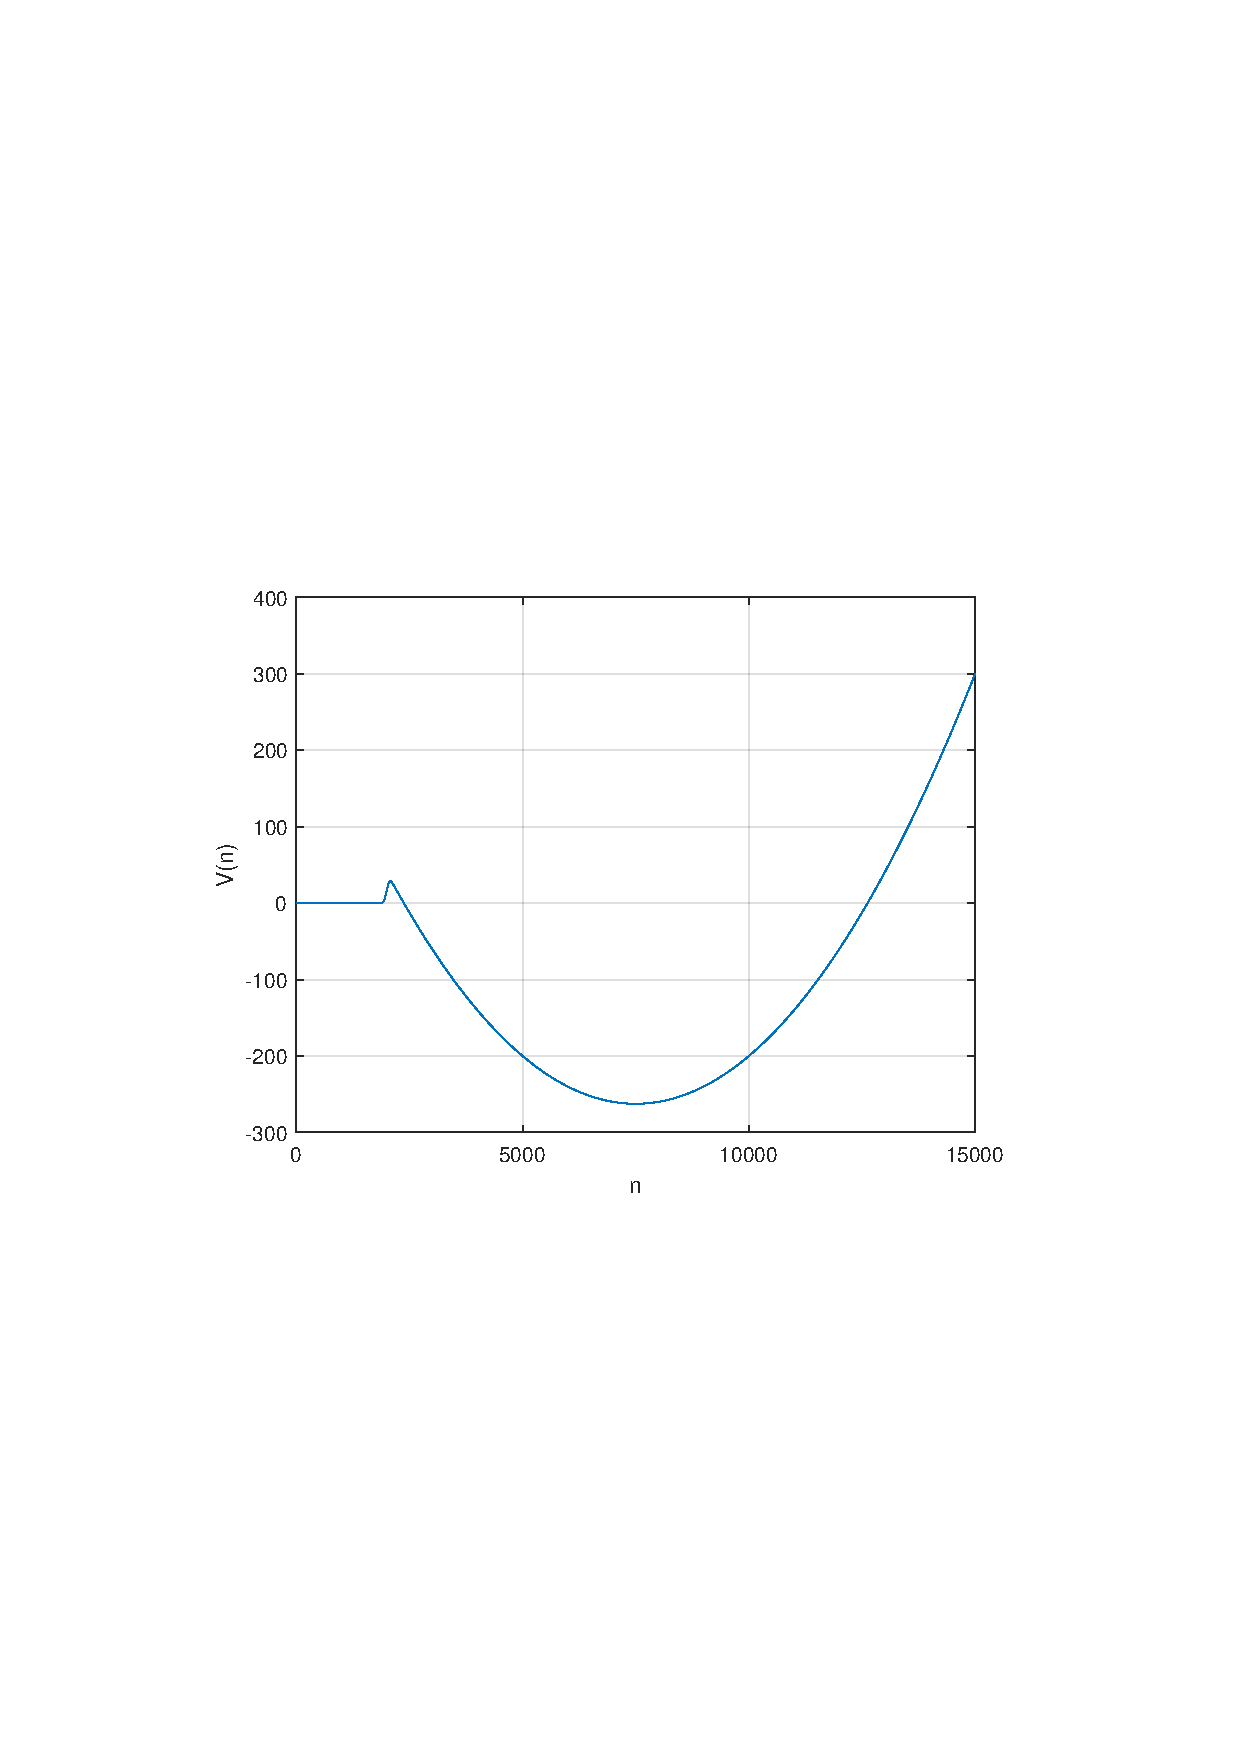
\includegraphics[width=0.8\textwidth,trim={3.09cm 9.295cm 3.09cm 9.295cm},clip]{fig/ex7_profit.pdf}
    \caption{利润$V$随购入报纸数量$n$变化的图像}
    \label{fig:ex7_profit}
\end{figure}

将$r$和$n$看作连续变量,则\Cref{eq:ex7_profit}可写作,
\begin{equation}
    V(n)=\int_0^n [(b-a) r-(a-c)(n-r)]f(r)dr + \int_n^{+\infty} (b-a)nf(r) dr
\end{equation}

注意这里$a$是关于$n$的函数,两边对$n$求导,化简得,
\begin{equation}
    V'(n) = \int_0^n \left(\frac{2An}{K}-A+c\right) f(r) dr + \int_n^{+\infty} \left(\frac{2An}{K}-A+b\right)f(r)dr
\end{equation}

令$V'(n)=0$,得到,
\begin{equation}
    \frac{\int_0^n f(r)dr}{\int_n^{+\infty} f(r)dr} = \frac{-2An+AK-bK}{2An-AK+cK}
\end{equation}

考虑到均值$\mu$比标准差$\sigma$大得多时,有$\int_0^n f(r)dr \approx \int_{-\infty}^n f(r)dr$,由对称性可知$\int_n^{+\infty} f(r)dr = 1-\int_{-\infty}^n f(r)dr$,因此得到,
\begin{equation}\label{eq:ex7_model}
    \int_{-\infty}^n f(r) dr = \frac{2An-AK+bK}{K(b-c)}
\end{equation}

\Cref{eq:ex7_model}即为本题的模型。

\paragraph{算法实现} \Cref{eq:ex7_model}是一个超越方程,无解析解,可采用\texttt{fzero}命令求解方程,采用\texttt{normcdf}命令计算正态分布的累积分布函数。

\subsubsection{程序}

请参见附录\ref{sec:ex7_code}。

\subsubsection{计算结果}

取初值为$n_0=2000$,计算得到最优购入报纸份数为$n=1968$。

\subsubsection{结果分析}

当限制$0 \le n \le 5000$时,批发价格$a$的取值范围为$0.45 \le a \le 0.5$,此时始终满足$c \le a \le b$,且批发价格与回收价格之间至少有0.1的差价,这是符合实际情况的。在这种限制下,求得的结果为全局最大值,可以作为实际应用的参考。

\subsubsection{结论}

为了获得最大利润,报童每天购进的报纸数应为1968份。


\subsection{Chap13-Ex9 洗衣粉泡沫(计算题)}

% 10. 轧钢有两道工序:粗轧和精轧。粗轧钢坯时由于各种随机因素的影响,得到的钢材的长度呈正态分布,其均值可由轧机调整,而方差是设备精度决定的,不能改变;精轧时将粗轧得到的钢材轧成规定的长度(可以认为没有误差)。如果粗轧后的钢材长度大于规定长度,精轧时要把多出的部分轧掉,造成浪费;如果粗轧后的钢材长度已经小于规定长度,则整根报废,浪费更大。问题是已知钢材规定的长度l 和粗轧后的钢材长度的均方差sigma,求可以调整的粗轧时钢材长度的均值m,使总的浪费最小。试从以下两种目标函数中选择一个,在l=2m,sigma=20cm 条件下求均值m:
% 1)每粗轧一根钢材的浪费最小;
% 2)每得到一根规定长度钢材的浪费最小。

\subsubsection{算法设计}

\paragraph{模型建立} 由题意,钢材的规定长度为$l$,粗轧得到的钢材长度服从正态分布$N(m,\sigma^2)$,记其概率密度函数为$f(x)$,累积分布函数为$F(x)$。

对于第1个目标函数,每粗轧一根钢材的浪费长度为,
\begin{equation}
    u(m) = \int_{-\infty}^l xf(x)dx + \int_l^{+\infty} (x-l)f(x)dx = m - l(1-F(l))
\end{equation}

对于第2个目标函数,每得到一根规定长度钢材的浪费长度为,
\begin{equation}
    v(m) = \frac{u(m)}{1-F(l)} = \frac{m}{1-F(l)} - l
\end{equation}

分别求出最佳均值$m$,使得$u(m)$和$v(m)$取最小值即可。

\paragraph{算法实现} 对于累积分布函数,可采用\texttt{normcdf}命令,对于最小值求解,可采用\texttt{fminunc}命令。

\subsubsection{程序}

请参见附录\ref{sec:ex9_code}。

\subsubsection{计算结果}

为了生产出合格的钢材并减少浪费,最佳均值$m$应当在2附近,首先画出区间[2,3]中的$u(m)$和$v(m)$图像,如\Cref{fig:ex9_waste}。可以看出,最小值在$m=2.3$附近,因此将其作为初值进行求解。

\begin{figure}[H]
    \centering
    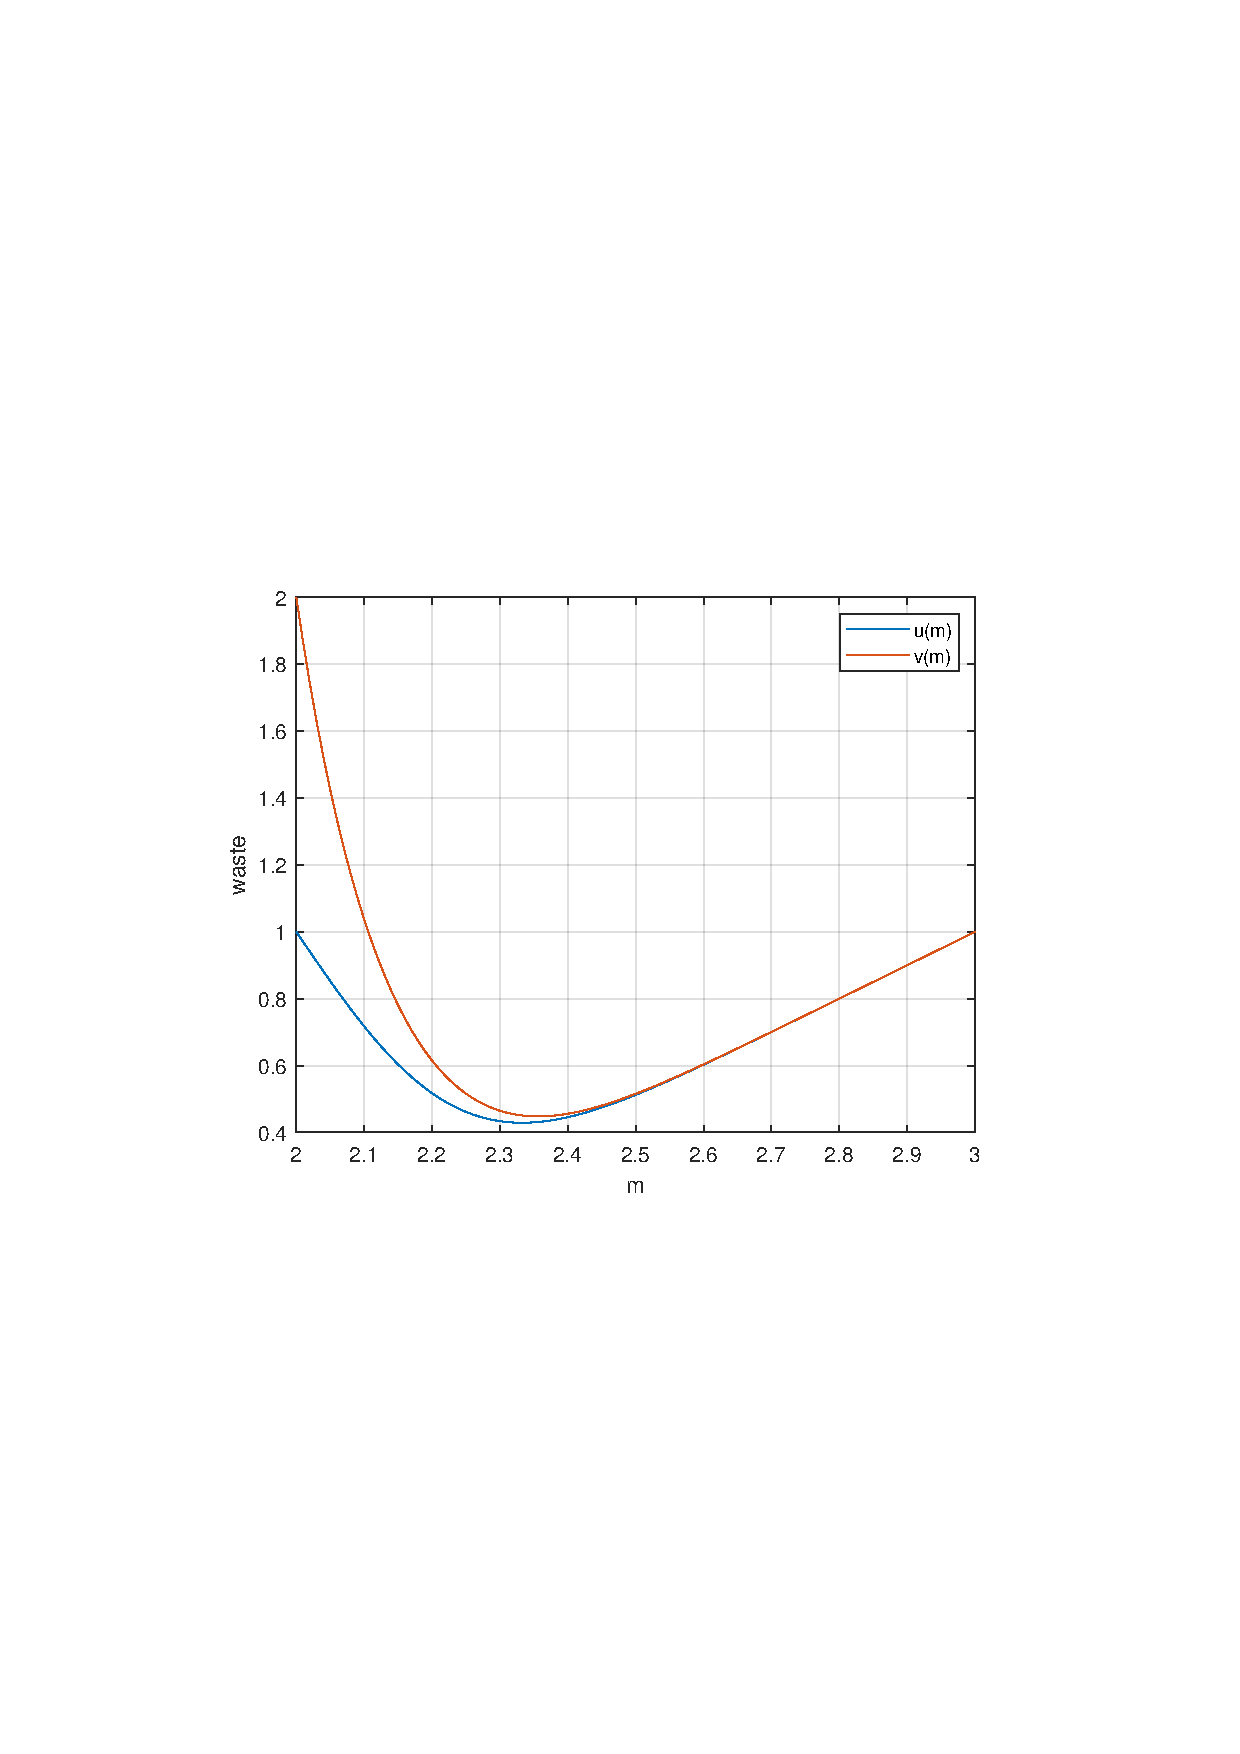
\includegraphics[width=0.8\textwidth,trim={3.09cm 9.295cm 3.09cm 9.295cm},clip]{fig/ex9_waste.pdf}
    \caption{两种目标函数的图像}
    \label{fig:ex9_waste}
\end{figure}

对于第1个目标函数,求解得到$m=2.3327$,此时浪费长度最小,为$u(m)=0.4289$。

对于第2个目标函数,求解得到$m=2.3562$,此时浪费长度最小,为$v(m)=0.4479$。

\subsubsection{结果分析}

由\Cref{fig:ex9_waste}可以看出,当$m$低于最优值时,粗轧得到钢管长度较短,导致整根报废的钢管数量较多,均摊到每根钢管的浪费长度较大;当$m$高于最优值时,粗轧得到的每根钢管长度较长,精轧时的浪费长度也较大;当$m$处于最优值时,达到了两者的平衡,此时平均浪费长度最小。

实际生产以利润为最终目标,生产利润往往与合格钢材的数量成正比,当生产每根合格钢材的浪费最小时,生产总利润最大,因此,在实际应用中,应当采用第2个目标函数。

\subsubsection{结论}

要求每粗轧一根钢材的浪费最小时,最优的粗轧钢材长度均值为2.3327米,此时平均浪费长度最小,为0.4289米。

要求每得到一根规定长度钢材的浪费最小时,最优的粗轧钢材长度均值为2.3562米,此时平均浪费长度最小,为0.4479米。


\subsection{Chap13-Ex13 Logistic模型(计算题)}

% 13.  Logistic 增长曲线模型和Gompertz增长曲线模型是计量经济学等学科中的两个常用模型,可以用来拟合销售量的增长趋势。
%     记Logistic 增长曲线模型为 y_t = L / (1 + a exp(-kt)),记Gompertz增长曲线模型为 y_t = L exp(-b exp(-kt)),这两个模型中L的经济学意义都是销售量的上限。表13.33中给出的是某地区高压锅的销售量(单位:万台),为给出此两模型的拟合结果,请考虑如下的问题:
% 1)	Logistic 增长曲线模型是一个可线性化模型吗。如果给定 L=3000,是否是一个可线性化模型,如果是,试用线性化模型给出参数a和k的估计值。
% 2)	利用1)所得到的a和k的估计值和L=3000作为Logistic模型的拟合初值,对Logistic模型做非线性回归。
% 3)	取初值L(0)=3000, b(0)=30, k(0)=0.4,拟合Gompertz模型。并与Logistic 模型的结果进行比较。

\subsubsection{算法设计}

\paragraph{第(1)问} Logistic增长曲线模型如下,
\begin{equation}
    y_t = \frac{L}{1 + a e^{-kt}}
\end{equation}

当参数$L,a,k$均未知时,该模型不是一个可线性化模型。当给定$L=3000$时,则是一个可线性化模型,可转化为,
\begin{equation}
    \ln\left(\frac{L}{y_t} - 1\right) = \ln a - kt
\end{equation}

其中$a,k$为待估参数。上式左端为因变量,记为$y$,自变量为$t$,令$\beta_0 = \ln a$且$\beta_1 = -k$,则上式可表示为$y = \beta_0 + \beta_1 t$。在MATLAB中,可采用\texttt{regress}命令进行线性回归。

\paragraph{第(2)问} 利用第(1)问所得到的$a$和$k$的估计值和$L=3000$作为Logistic模型的拟合初值,对Logistic模型做非线性回归。在MATLAB中,可采用\texttt{nlinfit}命令进行非线性回归。

\paragraph{第(3)问} Gompertz模型定义如下,
\begin{equation}
    y_t = L e^{-b e^{-kt}}
\end{equation}

取初值$L_0=3000, b_0=30, k_0=0.4$,用\texttt{nlinfit}命令进行非线性回归分析。

\subsubsection{程序}

请参见附录\ref{sec:ex13_code}。

\subsubsection{计算结果}

\paragraph{第(1)问} 经过计算,得到回归模型参数如\Cref{tab:ex13_logistic_linear}。

\begin{table}[H]
    \centering
    \caption{Logistic回归模型}
    \label{tab:ex13_logistic_linear}
    \begin{tabular}{|c|c|c|}
        \hline
        回归系数 & 估计值 & 置信区间\\
        \hline
        \hline
        \(\beta_0\) & 3.8032 & [3.5765, 4.0299]\\
        \hline
        \(\beta_1\) & -0.4941 & [-0.5262, -0.4621]\\
        \hline
        \multicolumn{3}{|c|}{$R^2=0.9905, \quad F=1150.7545, \quad p=0.0000, \quad s^2=0.0386$}\\
        \hline
    \end{tabular}
\end{table}

计算参数$a,k$的估计值,
\begin{equation}
    \hat{a} = e^{\hat{\beta}_0} = 44.8463, \quad \hat{k} = -\hat{\beta}_1 = 0.4941
\end{equation}

画出拟合曲线,如\Cref{fig:ex13_logistic_linear},经过计算,其剩余标准差为$s=5053.0508$。

\begin{figure}[H]
    \centering
    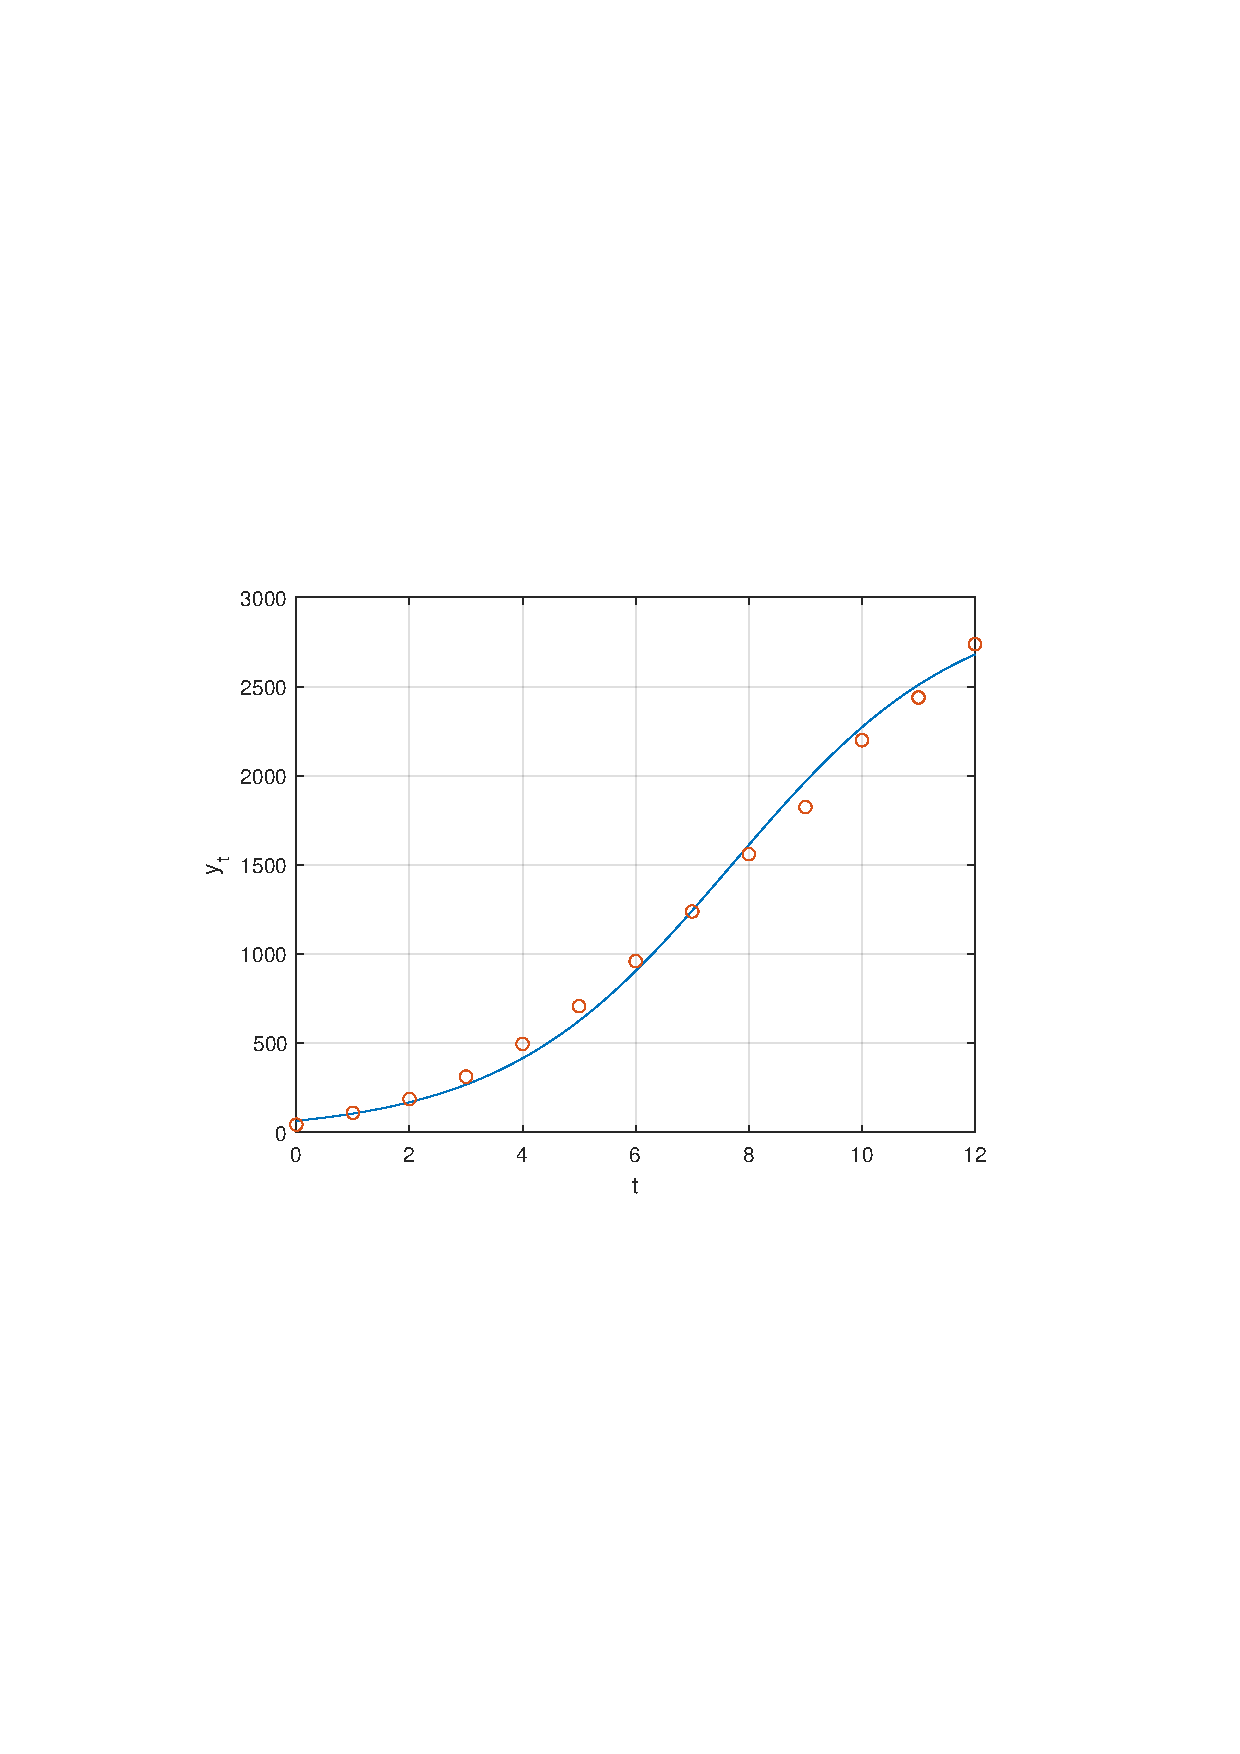
\includegraphics[width=0.8\textwidth,trim={3.09cm 9.295cm 3.09cm 9.295cm},clip]{fig/ex13_logistic_linear.pdf}
    \caption{Logistic线性回归模型拟合曲线}
    \label{fig:ex13_logistic_linear}
\end{figure}

\paragraph{第(2)问} 由第(1)问计算结果,可得非线性拟合的初值为$L_0 = 3000, a_0 = 44.8463, k_0 = 0.4941$,经过非线性回归,得到回归系数为,
\begin{equation}
    \hat{L} = 3260.4185, \quad \hat{a} = 30.5351, \quad \hat{k} = 0.4148
\end{equation}

画出拟合曲线,如\Cref{fig:ex13_logistic_nonlinear},其剩余标准差为$s=1765.1289$,模型的拟合效果比线性回归模型更好。

\begin{figure}[H]
    \centering
    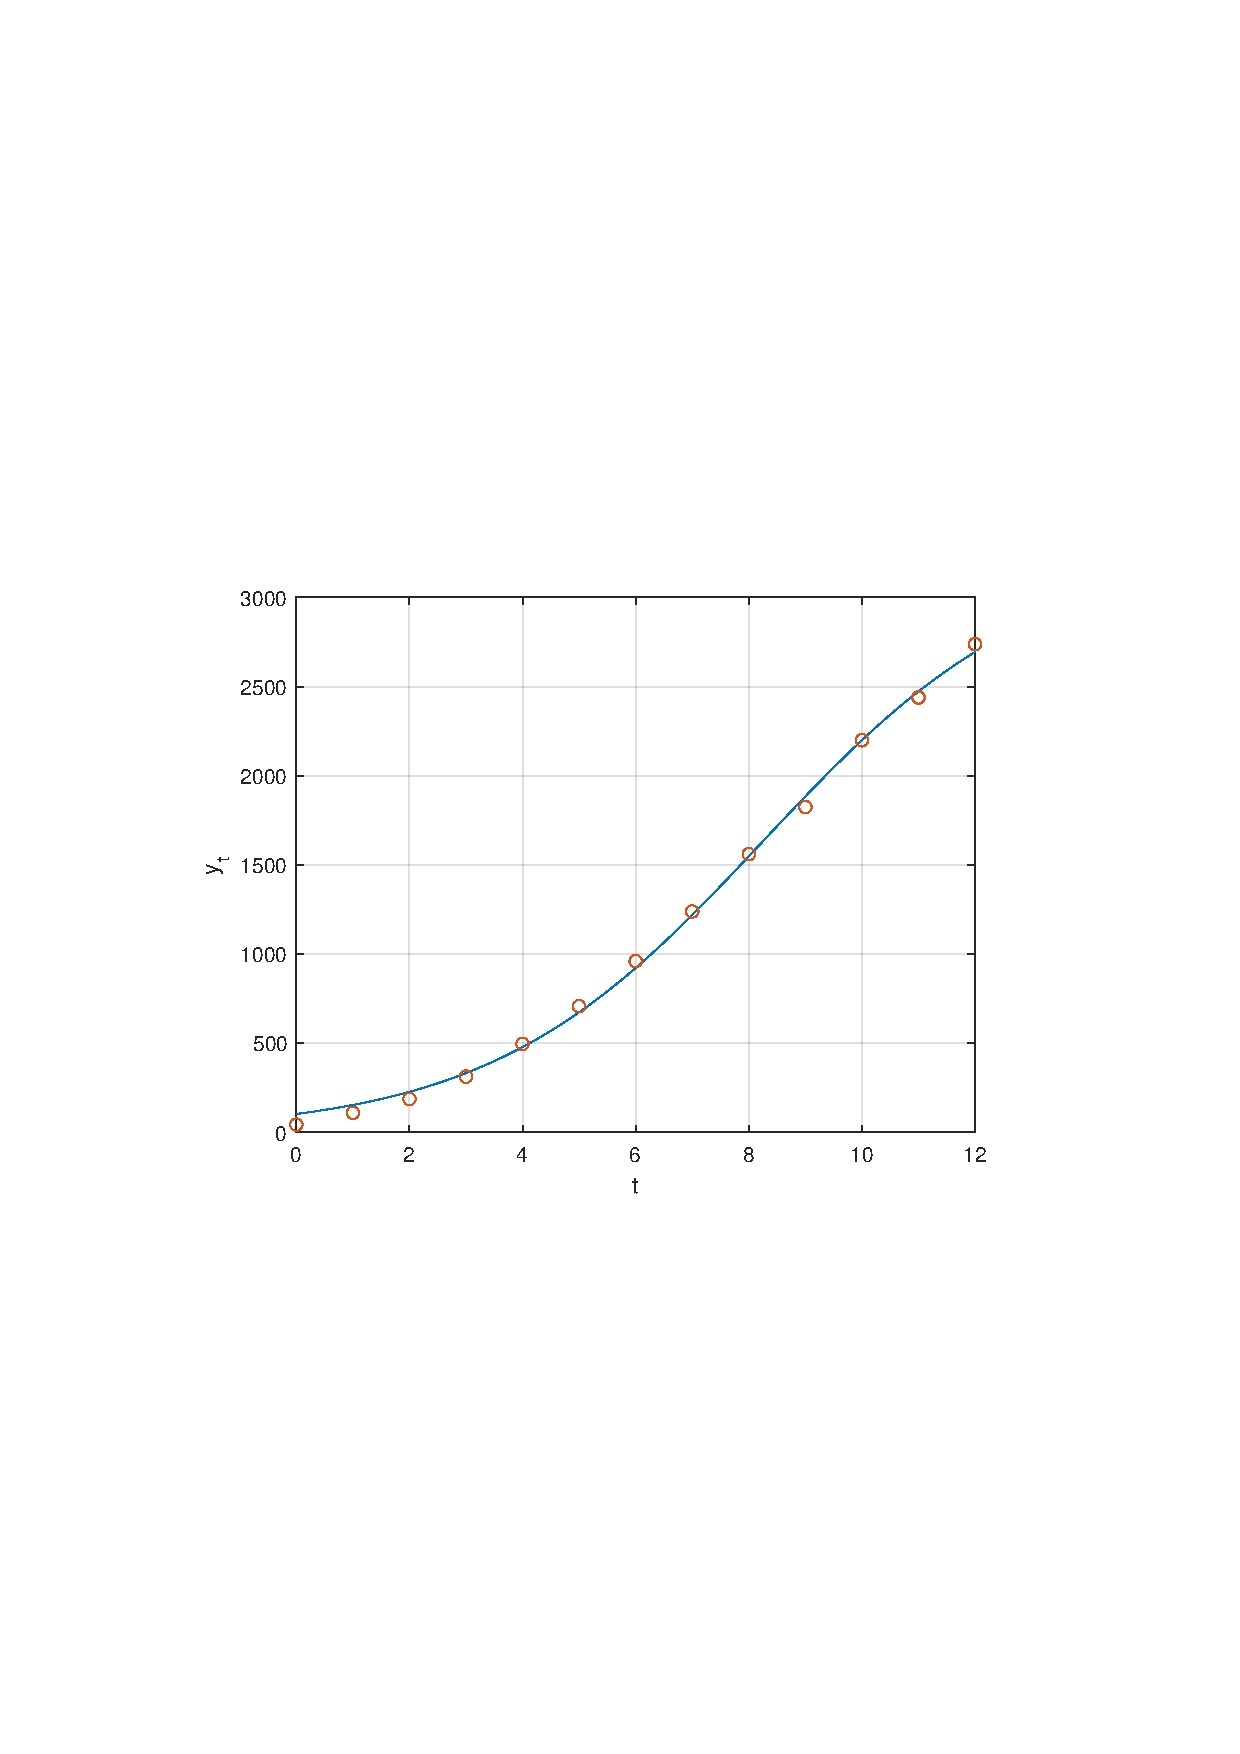
\includegraphics[width=0.8\textwidth,trim={3.09cm 9.295cm 3.09cm 9.295cm},clip]{fig/ex13_logistic_nonlinear.pdf}
    \caption{Logistic非线性回归模型拟合曲线}
    \label{fig:ex13_logistic_nonlinear}
\end{figure}

\paragraph{第(3)问} 以$L_0=3000, b_0=30, k_0=0.4$作为初值,经过非线性回归,得到Gompertz模型参数的估计值为,
\begin{equation}
    \hat{L} = 4810.1269, \quad \hat{b} = 4.5920, \quad \hat{k} = 0.1747
\end{equation}

画出拟合曲线,如\Cref{fig:ex13_gompertz_nonlinear},其剩余标准差为$s=308.1378$,低于Logistic模型,说明Gompertz模型比Logistic模型的拟合效果更好。

\begin{figure}[H]
    \centering
    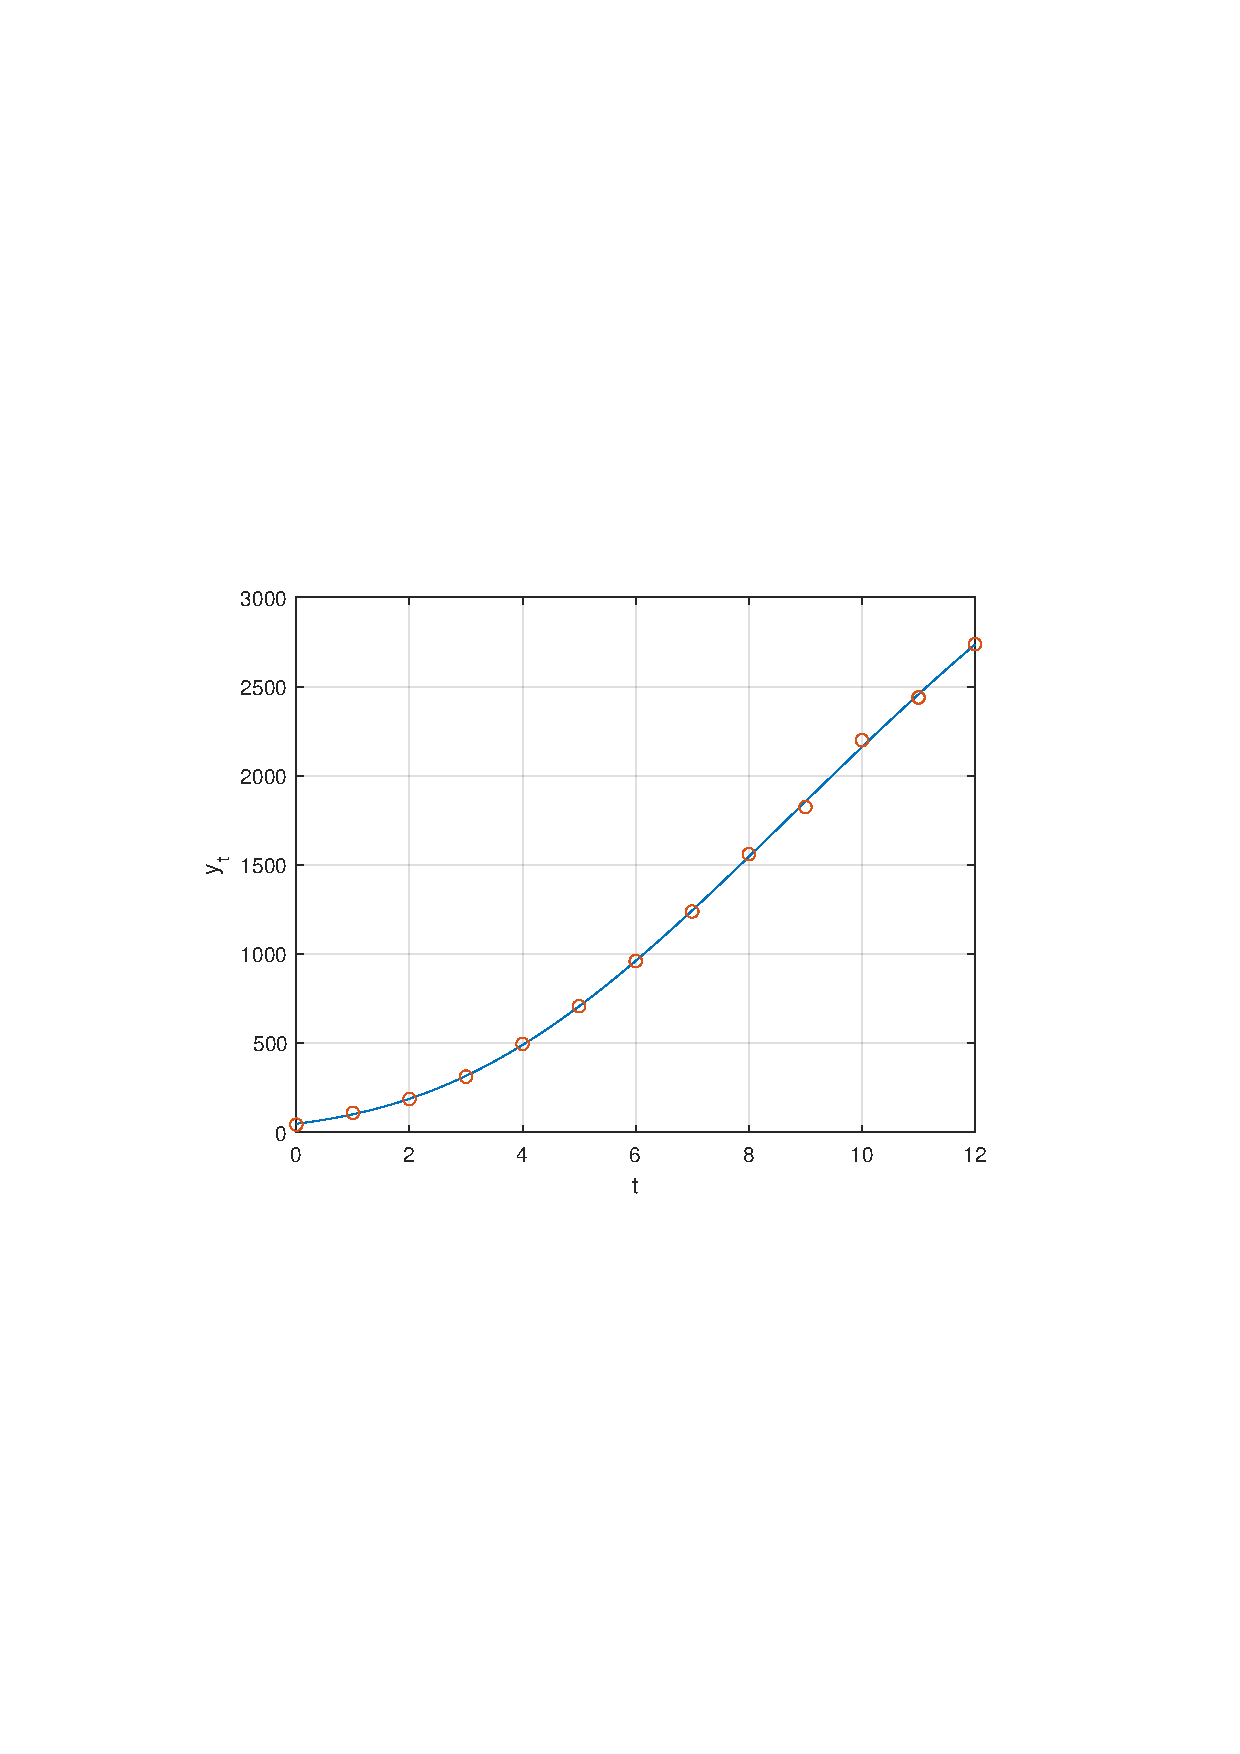
\includegraphics[width=0.8\textwidth,trim={3.09cm 9.295cm 3.09cm 9.295cm},clip]{fig/ex13_gompertz_nonlinear.pdf}
    \caption{Gompertz非线性回归模型拟合曲线}
    \label{fig:ex13_gompertz_nonlinear}
\end{figure}

\subsubsection{结果分析}

求解非线性回归模型时,选取合适的初值,可以降低计算量,加快收敛速度。如果模型可线性化,可以先求出线性化回归模型的参数估计值,将其作为初值,进一步求解非线性回归模型。

\subsubsection{结论}

Logistic增长曲线模型不是一个可线性化模型,如果给定$L=3000$,则是一个可线性化模型,用线性化模型给出参数$a$和$k$的估计值为$\hat{a} = 44.8463$和$\hat{k} = 0.4941$。

将上述$a$和$k$的估计值和$L=3000$作为Logistic模型的拟合初值,对Logistic模型做非线性回归,得到$\hat{L} = 3260.4185, \hat{a} = 30.5351, \hat{k} = 0.4148$。

取初值$L_0=3000, b_0=30, k_0=0.4$,拟合Gompertz模型,得到$\hat{L} = 4810.1269, \hat{b} = 4.5920, \hat{k} = 0.1747$,与Logistic模型相比,Gompertz模型的拟合效果更好。


\section{收获与建议}

在本次实验中,我掌握了回归分析的基本原理,用回归分析方法建立了实际问题的模型,并用MATLAB进行求解,在解决实际问题的过程中,我对数学方法的原理和应用有了更深刻的理解。

感谢老师和助教在这个学期的付出,我在这门课上收获颇丰,学到了很多应用数学的理论知识,掌握了用数学建模解决实际问题的基本方法,也锻炼了编程实践的能力。在以后的课程中,希望助教能对每次的实验进行详细的解答,希望老师在课堂上介绍更多数学应用的前沿知识。

\section{附录:程序代码}

\subsection{Chap13-Ex7}\label{sec:ex7_code}

\lstinputlisting[language=Matlab]{../src/ex7.m}

\subsection{Chap13-Ex9}\label{sec:ex9_code}

\lstinputlisting[language=Matlab]{../src/ex9.m}

\subsection{Chap13-Ex13}\label{sec:ex13_code}

\lstinputlisting[language=Matlab]{../src/ex13.m}

\end{document}